\documentclass[]{article}
\usepackage[UTF8]{ctex}
\usepackage[a4paper,left=10mm,right=10mm,bottom=10mm,top=10mm]{geometry}
\usepackage{graphicx}
\usepackage{float}
\usepackage{amsmath,amsfonts,amssymb,amsthm}
\usepackage{array,color}
%opening
\title{计算机科学中的数学基础Exercise15}
\author{陈昱衡 521021910939}
\date{\today}

\begin{document}

\maketitle


\section*{Warmup7}
\begin{figure}[H]
    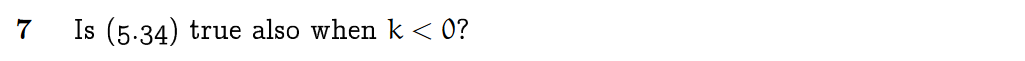
\includegraphics[scale = 0.6]{2023-04-03-17-14-54.png}
\end{figure}
根据之前证明过的结论:
\begin{figure}[H]
    \centering
    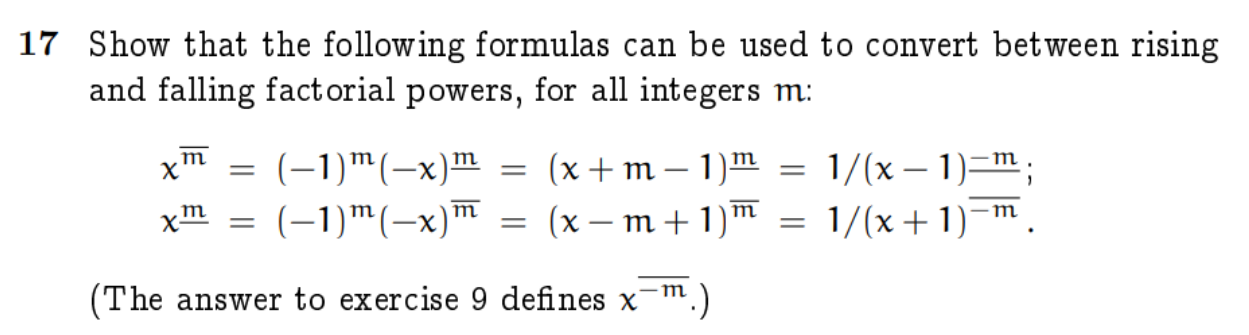
\includegraphics[scale = 0.3]{2023-04-03-23-37-43.png}
\end{figure}
可知,对于本题,将$k$换为$-k$,有
\begin{equation}
    r^{\underline{-k}}(r-\frac{1}{2})^{\underline{-k}} = \frac{1}{r^{\bar{k}}}\frac{1}{(r+\frac{1}{2})^{\bar{k}}}\\
\end{equation}
同时也有,\begin{equation}
    r^{\bar{k}}(r+\frac{1}{2})^{\bar{k}} = \frac{(2r)^{\bar{2k}}}{2^{2k}}
\end{equation}


\section*{Warmup8}
\begin{figure}[H]
    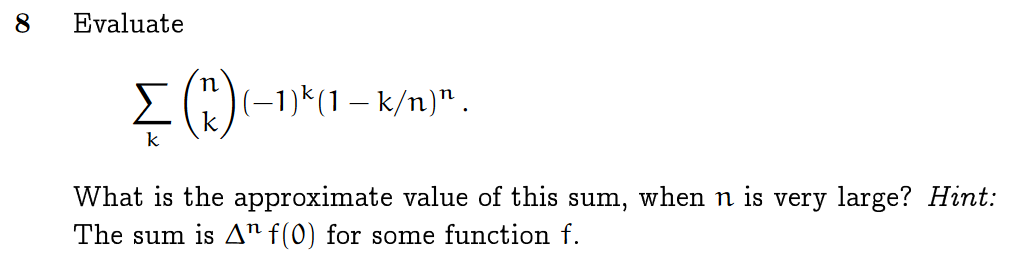
\includegraphics[scale = 0.6]{2023-04-03-17-16-17.png}
\end{figure}
由提示,取$f(k) = (\frac{k}{n} - 1)^{n}$,求n阶导,有
其0次项系数为$n^{-n}$.\par 
再由5.40中的结论,这个合式为
\begin{equation}
    \frac{n!}{n^n}
\end{equation}
当n趋近于无穷时,由斯特林公式,
\begin{equation}
    \frac{n!}{n^n} = \frac{\sqrt{2\pi n}}{e^n}.
\end{equation}

\section*{Basics14}
\begin{figure}[H]
    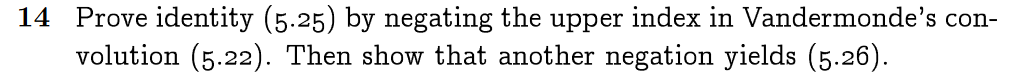
\includegraphics[scale = 0.6]{2023-04-03-17-17-40.png}
\end{figure}
首先观察求和下标,可以发现,题目中对$k \le l$求和就相当于5.25中对所有k求和。因为$\binom{m}{k}$当$k <0$是为0.\par 
故,有
\begin{align}
    \sum_{k \le l} \binom{l-k}{m}\binom{s}{k-n}(-1)^{k} &= \sum_{k}(-1)^{l-k-m}\binom{-m-1}{l-k-m}\binom{s}{k-n}\\
    &=\binom{s-m-l}{l-m-n}(-1)^{l+m}
\end{align}
将s使用$-1-n-q$替换即可得5.26\par 

\section*{Warmup15}
\begin{figure}[H]
    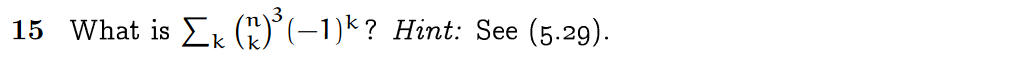
\includegraphics[scale = 0.6]{2023-04-03-17-17-56.png}
\end{figure}
根据式(5.29),观察结论,可以发现,可以令$a=b=c=\frac{n}{2}$.
\par 
若n为奇数,显然,原式和为0.\par 
若n为偶数,将$s=b=c=\frac{n}{2}$代入5.29,即有
\begin{equation}
    \sum_{k}\binom{n}{k}(-1)^k = (-1)^{\frac{n}{2}}(\frac{\frac{3n}{2} !}{\frac{m}{2} !}^{3})
\end{equation}


\end{document}